\clearpage

\section{Auswertung}
\label{sec:Auswertung}


\subsection{Kennlinien und Sättigungsstrom}
\label{subsec:kennlinien}
Es werden Kennlinien bei verschiedenen Heizleistungen aufgenommen und ausgewertet. Der Sättigungsstrom $I_S$, dem sich die $I$-Werte annähern, wird abgeschätzt.

\begin{table}
 \centering
 \caption{Messdaten bei einer Heizspannung von $2V$ und einem Heizstrom von $5A$.}
 \label{tab:daten1}
 \begin{tabular}{|c c|}  
 \toprule
I in $mA$ & U in $V$\\
\midrule
0.125 & 30\\
0.130 & 35\\
0.139 & 40\\
0.141 & 45\\
0.142 & 50\\
0.144 & 55\\
0.143 & 60\\
0.135 & 70\\
0.138 & 80\\
0.139 & 90\\
0.140 & 100\\
\bottomrule
\end{tabular}
\end{table}


\begin{figure}[H]
  \centering
  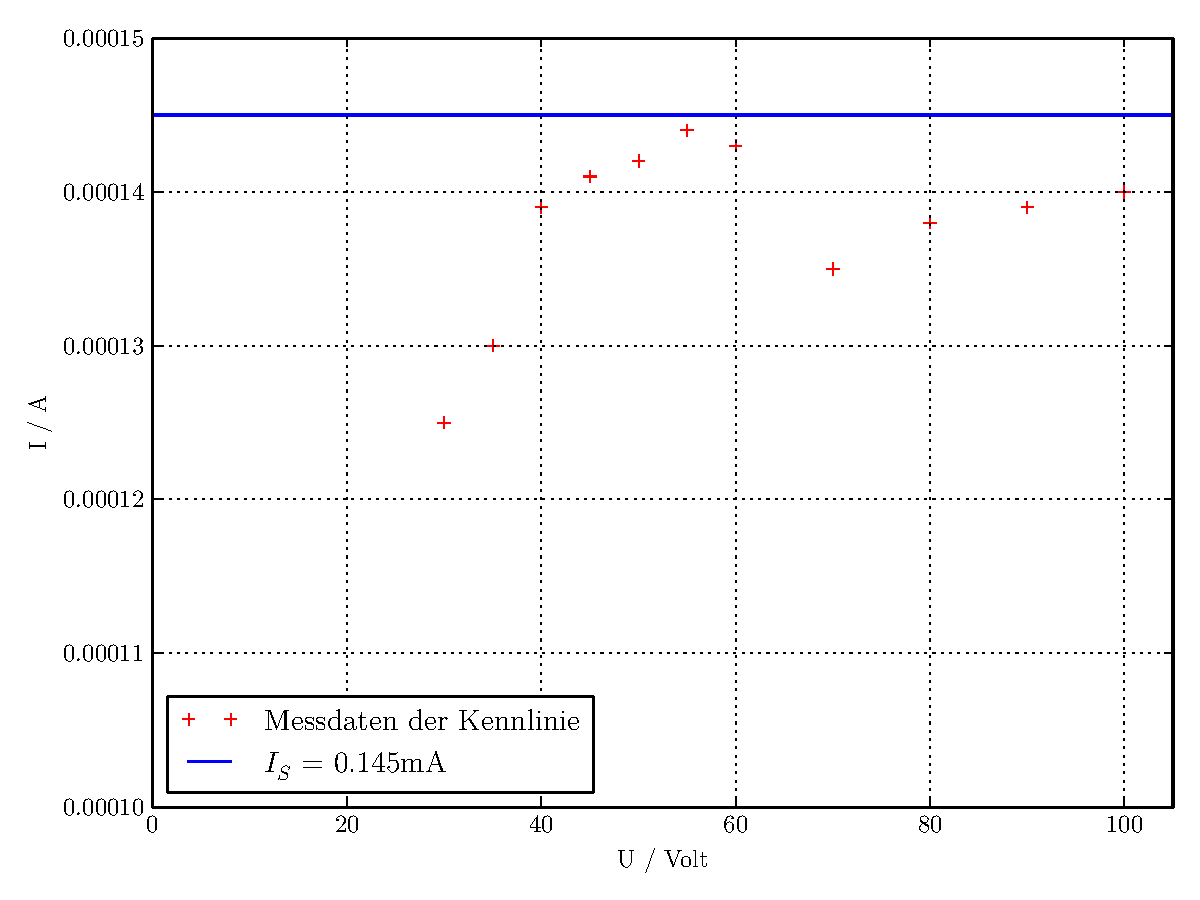
\includegraphics[width=0.9\textwidth]{build/Kennlinie1.pdf}
  \caption{Messdaten bei einer Heizspannung von 2V und einem Heizstrom von 5A \cite{sample}}
  \label{fig:kenn1}
\end{figure}
Bei den beschriebenen Heizungseigenschaften (Abb. \ref{fig:kenn1}) liegt der Sättigungsstrom bei 
\begin{equation}
I_S = 0.145 \mathrm{mA}.
\label{eq:kenn1ergebnis}
\end{equation}

\begin{table}
 \centering
 \caption{Messdaten bei einer Heizspannung von $2.2V$ und einem Heizstrom von $5.5A$.}
 \label{tab:daten2}
 \begin{tabular}{|c c|}  
 \toprule
I in $mA$ & U in $V$\\
\midrule
0.355 & 30\\
0.439 & 35\\
0.498 & 40\\
0.549 & 45\\
0.594 & 50\\
0.633 & 55\\
0.709 & 60\\
0.716 & 70\\
0.734 & 80\\
0.735 & 85\\
\bottomrule
\end{tabular}
\end{table}


\begin{figure}[H]
  \centering
  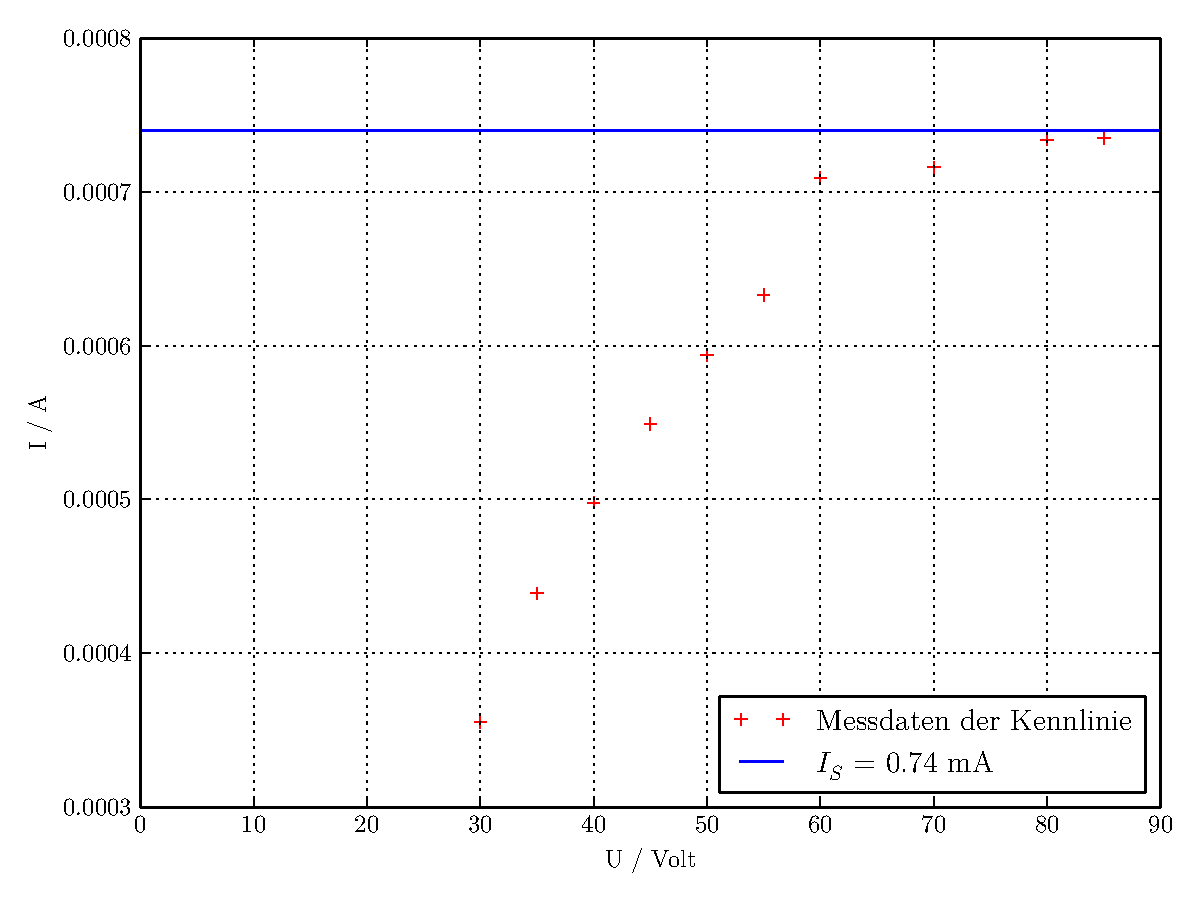
\includegraphics[width=0.8\textwidth]{build/Kennlinie2.pdf}
  \caption{Messdaten bei einer Heizspannung von 2.2V und einem Heizstrom von 5.5A \cite{sample}}
  \label{fig:kenn2}
\end{figure}
Bei den beschriebenen Heizungseigenschaften (Abb. \ref{fig:kenn2}) liegt $I_S$ bei 
\begin{equation}
I_S = 0.74 \mathrm{mA}.
\label{eq:kenn2ergebnis}
\end{equation}

\begin{table}
 \centering
 \caption{Messdatentabelle bei einer Heizspannung von $2.4V$ und einem Heizstrom von $6A$.}
 \label{tab:daten4}
 \begin{tabular}{|c c|| c c |}  
 \toprule
I in $mA$ & U in $V$ & I in $mA$ & U in $V$\\
\midrule
0.034	&0   &1.84	 &100\\
0.035	&5	 &1.97	 &110\\
0.092	&10	 &2.07	 &120\\
0.182	&15	 &2.15	 &130\\
0.26	&20	 &2.2 	 &140\\
0.362	&25	 &2.24	 &150\\
0.459	&30	 &2.25	 &160\\
0.574	&35	 &2.28	 &170\\
0.708	&40	 &2.3	   &180\\
0.831	&45	 &2.32	 &190\\
0.991	&50	 &2.33	 &200\\
1.069	&55	 &2.33	 &210\\
1.14	&60	 &2.34	 &220\\
1.34	&70	 &2.35	 &230\\
1.54	&80	 &2.36	 &240\\
1.7	  &90	 &2.37	 &250\\
\bottomrule
\end{tabular}
\end{table}


\begin{figure}[H]
  \centering
  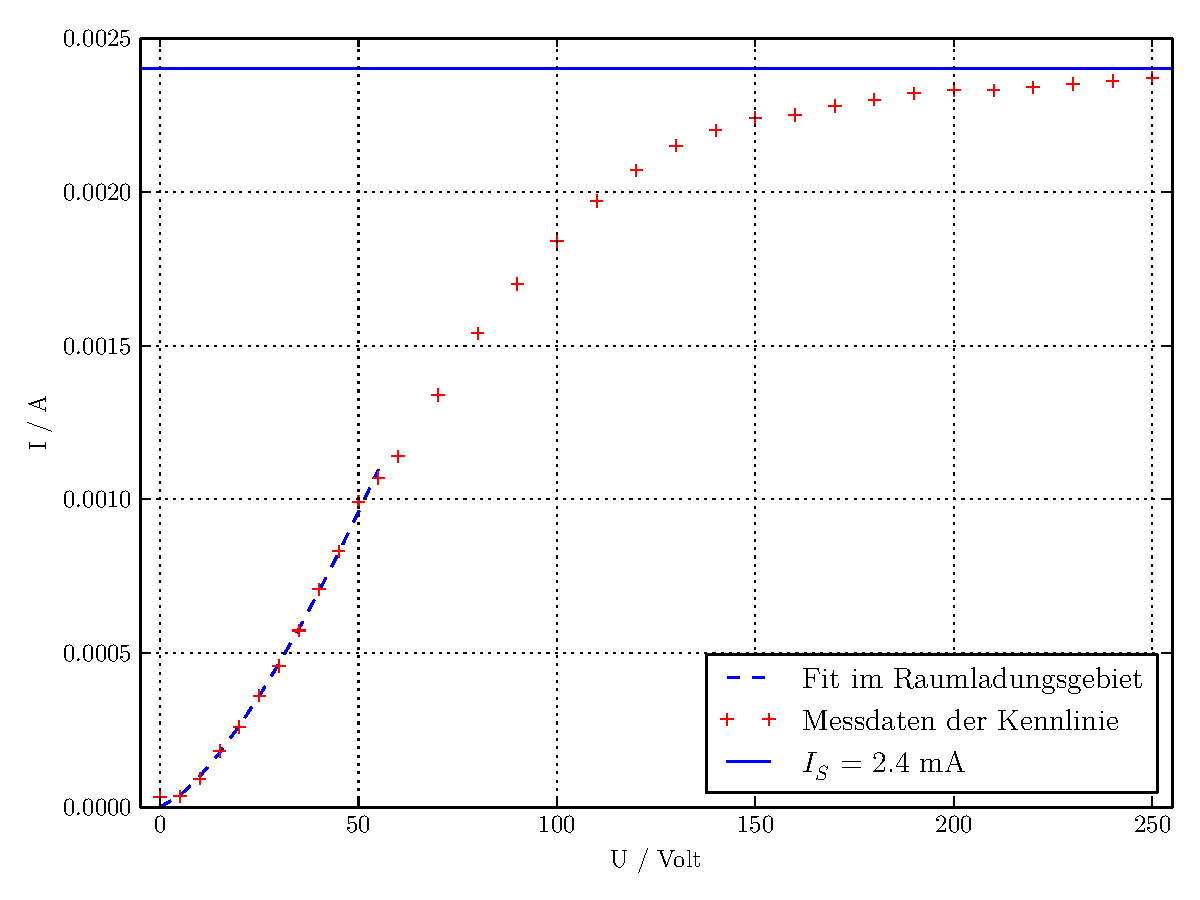
\includegraphics[width=0.8\textwidth]{build/Kennlinie4.pdf}
  \caption{Messdaten bei einer Heizspannung von 2.4V und einem Heizstrom von 6A \cite{sample}}
  \label{fig:kenn4}
\end{figure}
Bei den beschriebenen Heizungseigenschaften (Abb. \ref{fig:kenn4}) liegt der Strom bei 
\begin{equation}
I_S = 2.4 \mathrm{mA}.
\label{eq:kenn4ergebnis}
\end{equation}
Der Raumladungsbereuch wurde nach Abbildung \ref{fig:6} abgeschätzt. In diesem Bereich wird
gegenüber den Daten ein Fit angelegt. Dies geschieht nach der Gleichung \eqref{eq:langmuir}. Der Exponent der Spannung U war dabei
der zu bestimmende Fitparameter der Fitfunktion $I (U) = \mathrm{const} \cdot \frac{\mathrm{U}^b}{\mathrm{a}^2}$ . Er wurde mit NumPy \cite{numpy} als 1.407 bestimmt während a bei 7.73 liegt.



\subsection{Das Anlaufstromgebiet und die Temperatur}
\label{subsec:c}
Die Messdaten des Anlaufstromgebiets werden geplottet und es wird nach einer Spannungskorrektur eine Ausgleichskurve nach \eqref{eq:anlauf} angelegt.
\begin{figure}[H]
  \centering
  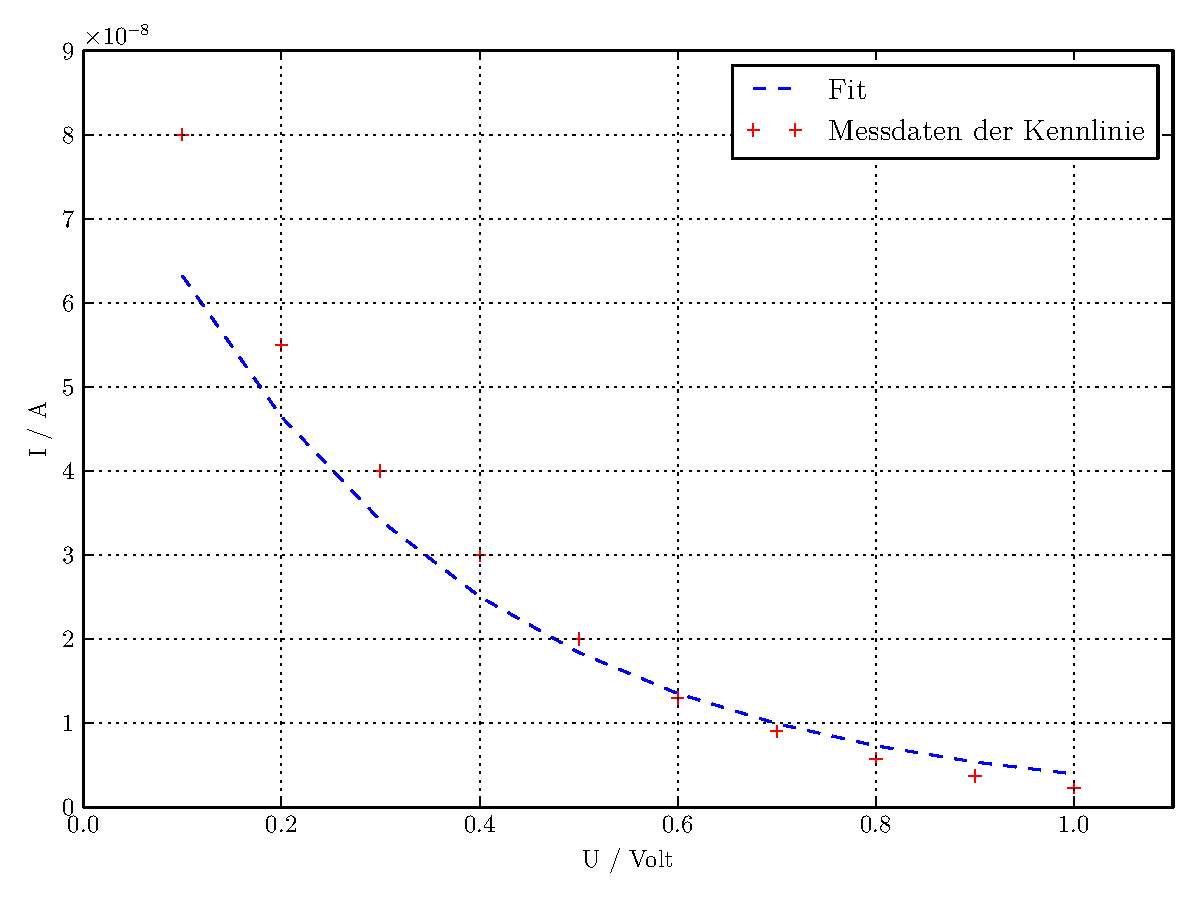
\includegraphics[width=0.9\textwidth]{build/Kennlinie3.pdf}
  \caption{Messdaten des Anlaufstromgebiets bei einer Heizspannung von 2.4V und einem Heizstrom von 6A \cite{sample}}
  \label{fig:kenn3}
\end{figure}
An die Daten legen wir eine Fitfunktion $I (U) =a \cdot e^{-b U}$. Mit den herausgefundenen Parametern $a= 8.6*10^-8 \pm 1.6*10^-9$ und $b=3.09 \pm 0.089$ wird mit Gleichung
\eqref{eq:anlauf} eine Temperatur von $3761.16 \mathrm{K} \pm 2.897 \%$ errechnet.


\subsection{Kathodentemperaturen}
\label{subsec:d}
Mit 
\begin{equation}
T = \sqrt[4]{\frac{I_H \cdot U_H - N_{WL}}{f \eta \sigma}}
\label{eq:kenn1ergebnis}
\end{equation}
\cite{sample} kann die Temperatur aus den gemessenen Wertepaaren in Unterkapitel \ref{subsec:kennlinien} errechnet werden.

So werden folgende Temperaturen gefunden.
\begin{table}
 \centering
 \caption{Temperaturen der Heizkathoden}
 \label{tab:datenaustritt}
 \begin{tabular}{|c c c|}  
 \toprule
$I_H$ / A & $U_H$ / U & Temperatur in $K$\\
\midrule
5A & 2V & $2048.87$\\
5.5A & 2.2V & $2159.16$\\
6A & 2.4V & $2263.24$\\
\bottomrule
\end{tabular}
\end{table}

\subsection{Austrittsarbeit}
\label{subsec:e}
Durch das Umstellen von Gl. \eqref{eq:richardson} ist es möglich, die Austrittsarbeit des verwendeten Materials 
(hier: Wolfram) auszurechnen. 

\begin{equation}
\label{eq:arbeit}
\end{equation}

Es ergeben sich folgende Daten.
\begin{table}
 \centering
 \caption{Austrittsarbeiten}
 \label{tab:datenaustritt}
 \begin{tabular}{|c c c|}  
 \toprule
$I_H$ / A & $U_H$ / U & Austrittsarbeit in $eV$\\
\midrule
5A & 2V & 3.82\\
5.5A & 2.2V & 3.73\\
6A & 2.4V & 3.71\\
\bottomrule
\end{tabular}
\end{table}